%; whizzy paragraph -pdf xpdf -latex ./whizzypdfptex.sh
%; whizzy-paragraph "^\\\\begin{frame}"
% latex beamer presentation.
% platex, latex-beamer $B$G%3%s%Q%$%k$9$k$3$H$rA[Dj!#(B 

%     Tokyo Debian Meeting resources
%     Copyright (C) 2009 Junichi Uekawa
%     Copyright (C) 2009 Nobuhiro Iwamatsu

%     This program is free software; you can redistribute it and/or modify
%     it under the terms of the GNU General Public License as published by
%     the Free Software Foundation; either version 2 of the License, or
%     (at your option) any later version.

%     This program is distributed in the hope that it will be useful,
%     but WITHOUT ANY WARRANTY; without even the implied warreanty of
%     MERCHANTABILITY or FITNESS FOR A PARTICULAR PURPOSE.  See the
%     GNU General Public License for more details.

%     You should have received a copy of the GNU General Public License
%     along with this program; if not, write to the Free Software
%     Foundation, Inc., 51 Franklin St, Fifth Floor, Boston, MA  02110-1301 USA

\documentclass[cjk,dvipdfmx,12pt]{beamer}
\usetheme{Tokyo}
\usepackage{monthlypresentation}
\usepackage{listings}

%  preview (shell-command (concat "evince " (replace-regexp-in-string "tex$" "pdf"(buffer-file-name)) "&")) 
%  presentation (shell-command (concat "xpdf -fullscreen " (replace-regexp-in-string "tex$" "pdf"(buffer-file-name)) "&"))
%  presentation (shell-command (concat "evince " (replace-regexp-in-string "tex$" "pdf"(buffer-file-name)) "&"))

%http://www.naney.org/diki/dk/hyperref.html
%$BF|K\8l(BEUC$B7O4D6-$N;~(B
\AtBeginDvi{\special{pdf:tounicode EUC-UCS2}}
%$B%7%U%H(BJIS$B7O4D6-$N;~(B
%\AtBeginDvi{\special{pdf:tounicode 90ms-RKSJ-UCS2}}

\title{Golang$B$G=q$+$l$?%D!<%k$r(B\\Debian$B%Q%C%1!<%8$K$9$k(B}
\subtitle{}
\author{$B$^$($@$3$&$X$$(B}
\date{2014$BG/(B4$B7n(B19$BF|(B}
\logo{\includegraphics[width=8cm]{image200607/openlogo-light.eps}}

\begin{document}
\lstset{ %
  backgroundcolor=\color{dancerlightblue},
  language=sh
}

\frame{\titlepage{}}

\begin{frame}{$B<+8J>R2p(B}
 \begin{itemize}
  \item[Debian:] blockdiag$B%7%j!<%:!"(Bdjango REST framework$B!"(B\\yrmcds$B$J$I$N%a%s%F%J(B
  \item[$B8@8l(B:] $B<g$K(BPython$B!#(B\\$B:G6a(BGolang$B$b;H$*$&$HJY6/Cf(B
  \item[$B2HDm(B:] $BG-0lI$(B($B!j(B)$B!"L<Fs?M!":J0l?M(B
  \item[$BJY6/2q(B:] $B$[$\(BDebian$BJY6/2q$N$_!#$G$b:#F|$OLsH>G/$V$j(B
  \item[$B;E;v(B:] Python$B$G(BLDAP$B$4$K$g$4$K$g$H$+!"(B\\django REST framework$B$G(BAPI$B3+H/$H$+(B
 \end{itemize}
\end{frame}

\begin{frame}{$B:#F|$NOC$NN.$l$HA0Ds(B}
\begin{itemize}
  \item Golang$B$N%D!<%k$r%Q%C%1!<%82=$7$h$&$H;W$C$?F05!(B
  \item Debian$B$G$N(BGolang$B$r;H$&J}K!(B
  \item Debian$B%Q%C%1!<%82=$KI,MW$J(BGolang$B$NCN<1(B
  \item $B%Q%C%1!<%82=$9$k$?$a$N$*:nK!(B
  \item Golang$B$N%D!<%k$r(BDebian$B%Q%C%1!<%8$K$9$k(B
\end{itemize}

$B"(A0Ds>r7o!'(B Sid$B$r=`Hw$9$k$3$H(B
\end{frame}


\begin{frame}{$B:#F|$NOC$NN.$l$HA0Ds(B}
\begin{itemize}
  \item \textcolor{red}{Golang$B$N%D!<%k$r%Q%C%1!<%82=$7$h$&$H;W$C$?F05!(B}
  \item Debian$B$G$N(BGolang$B$r;H$&J}K!(B
  \item Debian$B%Q%C%1!<%82=$KI,MW$J(BGolang$B$NCN<1(B
  \item $B%Q%C%1!<%82=$9$k$?$a$N$*:nK!(B
  \item Golang$B$N%D!<%k$r(BDebian$B%Q%C%1!<%8$K$9$k(B
\end{itemize}

$B"(A0Ds>r7o!'(B Sid$B$r=`Hw$9$k$3$H(B
\end{frame}

\begin{frame}{Serf$B$r;H$*$&$H;W$C$?$N$G(B}
  \begin{itemize}
  \item[0.] $B$d$j$?$$$H;W$C$F$$$k$3$H$r(BSerf$B$G$G$-$=$&!)(B
  \item[1.] main$B$K$J$$$N$G(BDebian$B%Q%C%1!<%8$r:n@.$9$C$+(B
  \item[2.] $B0MB84X78$N%Q%C%1!<%8$b8.JB$_%Q%C%1!<%82=I,MW!*(B
  \item[3.] $BA4It:n$C$?$1$IB?$$!*(Bpkg-go$B%A!<%`$K2CF~!*(B
  \item[4.] pkg-go$B$N%]%j%7!<8+$?$i!"%Q%C%1!<%8L>$J$I=$@5I,MW(B
  \item[5.] $B=$@5=*$o$C$?$N$G!"(BML$BEj9F$H(BITP$B$d$k$+!<"+%$%^%3%3(B
  \end{itemize}
\end{frame}

\begin{frame}{Debian$B%Q%C%1!<%82=$,I,MW$J$b$N$I$b(B($B"(;M3Q(B)}
\begin{figure}[H]
\begin{center}
  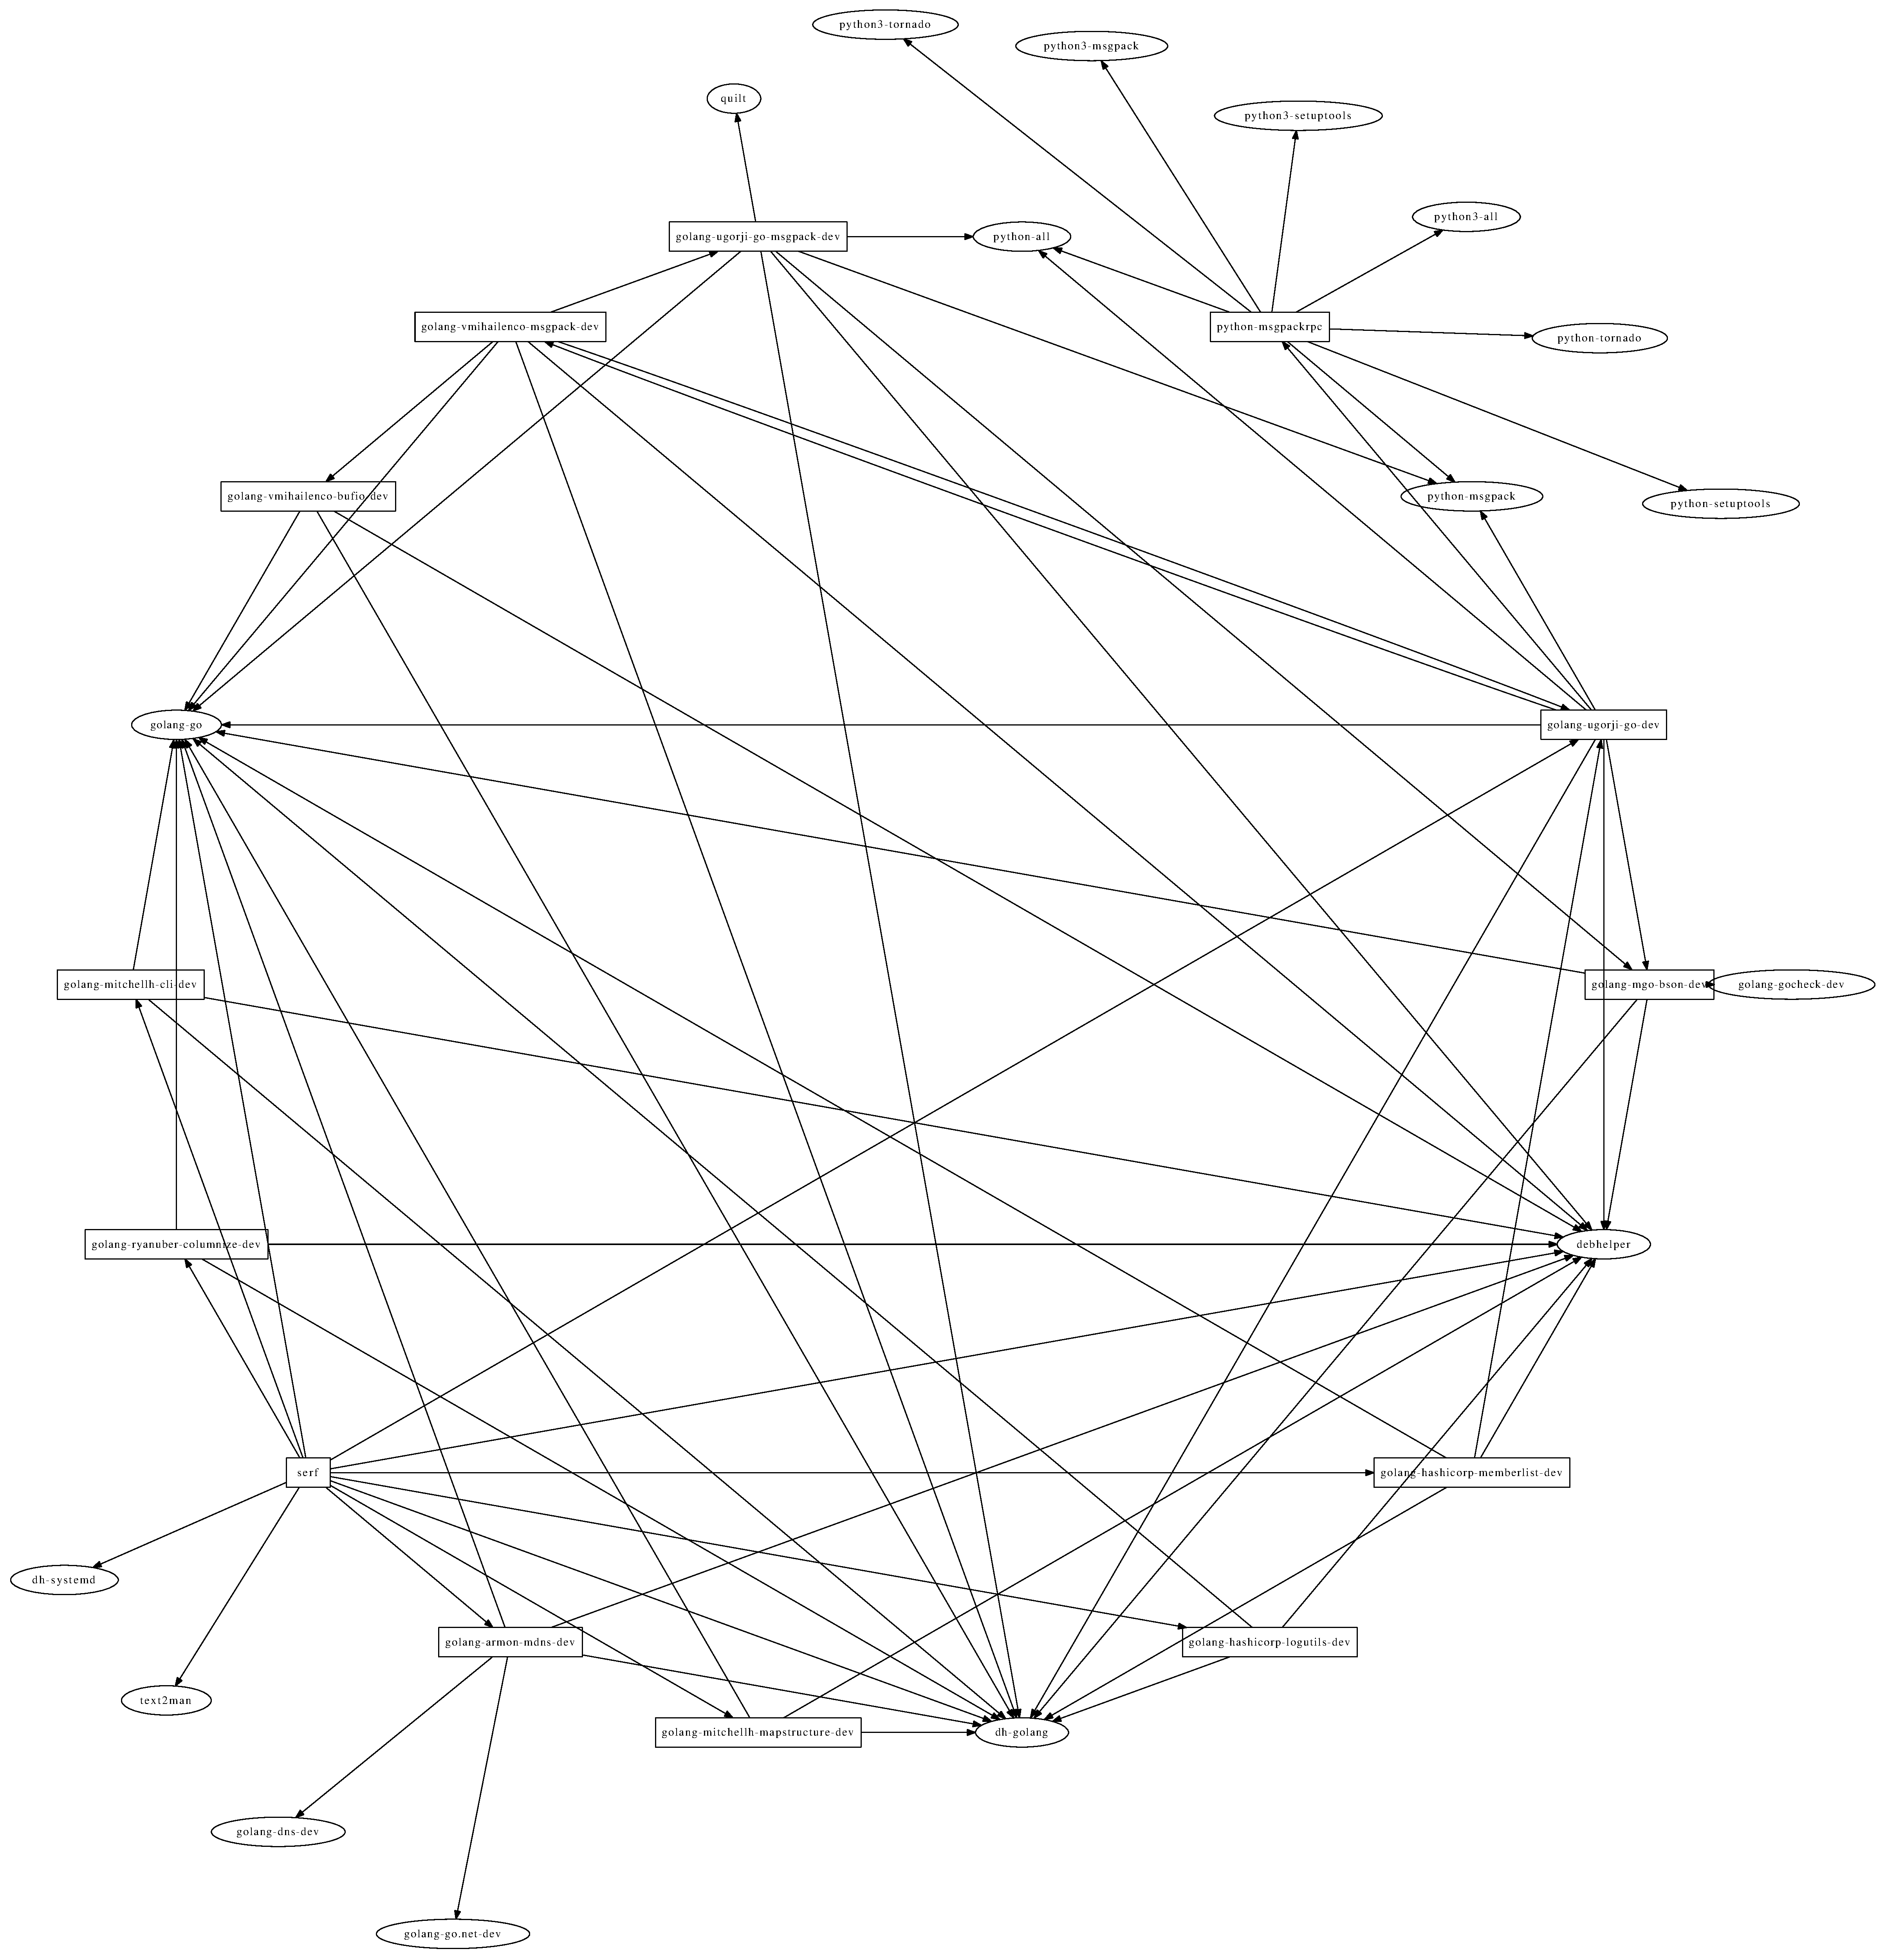
\includegraphics[width=0.7\hsize]{image201404/serf-dependency.eps}
 \label{fig:serf-dependencies}
\end{center}
\end{figure}
\end{frame}

\begin{frame}{$B!!(B}
\begin{itemize}
  \item Golang$B$N%D!<%k$r%Q%C%1!<%82=$7$h$&$H;W$C$?F05!(B
  \item \textcolor{red}{Debian$B$G$N(BGolang$B$r;H$&J}K!(B}
  \item Debian$B%Q%C%1!<%82=$KI,MW$J(BGolang$B$NCN<1(B
  \item $B%Q%C%1!<%82=$9$k$?$a$N$*:nK!(B
  \item Golang$B$N%D!<%k$r(BDebian$B%Q%C%1!<%8$K$9$k(B
\end{itemize}
\end{frame}

\begin{frame}[containsverbatim]{Debian$B$G$N(BGolang$B$N4D6-9=C[(B}
\begin{commandline}
$ sudo apt-get install golang
\end{commandline}
\end{frame}

\begin{frame}{$B%$%s%9%H!<%k$5$l$k%Q%C%1!<%8(B}
\begin{itemize}
\item golang-doc
\item golang-go
\item golang-go-linux-amd64 \footnote{amd64$B$N>l9g(B}
\item golang-go.tools
\item golang-src
\item libjs-jquery
\item javascript-common
\end{itemize}
\end{frame}


\begin{frame}{$B!!(B}
\begin{itemize}
  \item Golang$B$N%D!<%k$r%Q%C%1!<%82=$7$h$&$H;W$C$?F05!(B
  \item Debian$B$G$N(BGolang$B$r;H$&J}K!(B
  \item \textcolor{red}{Debian$B%Q%C%1!<%82=$KI,MW$J(BGolang$B$NCN<1(B}
  \item $B%Q%C%1!<%82=$9$k$?$a$N$*:nK!(B
  \item Golang$B$N%D!<%k$r(BDebian$B%Q%C%1!<%8$K$9$k(B
\end{itemize}
\end{frame}

\begin{frame}[containsverbatim]{Golang$B$N%3%s%Q%$%kJ}K!(B}
  hello world(hello.go)$B$rMQ0U(B
 \begin{commandline}
package main

import "fmt"

func main() {
  fmt.Println("Hello world.")
}
 \end{commandline}
\end{frame}

\begin{frame}[containsverbatim]{Golang$B$N%3%s%Q%$%kJ}K!(B}
  go build$B$G%3%s%Q%$%k(B
 \begin{commandline}
$ go build hello.go
 \end{commandline}
\end{frame}

\begin{frame}[containsverbatim]{Golang$B$N%3%s%Q%$%kJ}K!(B}
$B<B9T(B
 \begin{commandline}
$ ./hello
Hello world.
 \end{commandline}
\end{frame}

\begin{frame}[containsverbatim]{Golang$B$N%3%s%Q%$%kJ}K!(B}
$B@EE*%j%s%/$5$l$F$$$k$3$H$r3NG'(B
 \begin{commandline}
$ file hello
hello: ELF 64-bit LSB executable, x86-64, \
version 1 (SYSV), statically linked, not stripped
 \end{commandline}
\end{frame}

\begin{frame}[containsverbatim]{$BI8=`%i%$%V%i%j0J30$K0MB8$9$k>l9g(B}
\begin{itemize}
  \item $B4D6-JQ?t(BGOPATH$B$r@_Dj(B
  \item $BI8=`%i%$%V%i%j0J30$N(BGolang$B$N(BDebian$B%Q%C%1!<%8$O!"(B/usr/share/gocode$B$K%$%s%9%H!<%k$5$l$k(B
\end{itemize}
\begin{commandline}
$ export GOPATH=/usr/share/gocode
\end{commandline}
\end{frame}

\begin{frame}[containsverbatim]{$BI8=`%i%$%V%i%j0J30$K0MB8$9$k>l9g(B}
golang-dns-dev(Go$BMQ$N(BDNS$B%i%$%V%i%j(B)$B$r;H$C$F$_$k(B
\begin{commandline}
$ sudo apt-get install golang-dns-dev
$ dpkg -L golang-dns-dev
(snip)
/usr/share/gocode
/usr/share/gocode/src
/usr/share/gocode/src/github.com
/usr/share/gocode/src/github.com/miekg
/usr/share/gocode/src/github.com/miekg/dns
/usr/share/gocode/src/github.com/miekg/dns/zscan_rr.go
/usr/share/gocode/src/github.com/miekg/dns/zscan.go
\end{commandline}
\end{frame}

\begin{frame}[containsverbatim]{$BI8=`%i%$%V%i%j0J30$K0MB8$9$k>l9g(B}
Golang$B$N%D!<%k$G0MB8%Q%C%1!<%8$r%$%s%9%H!<%k>l9g(B
$B"(%f!<%6%G%#%l%/%H%j$K%$%s%9%H!<%k$9$kNc(B
\begin{commandline}
$ mkdir $HOME/gocode
$ export GOPATH=$HOME/gocode
$ go get github.com/miekg/dns
\end{commandline}
\end{frame}

\begin{frame}[containsverbatim]{$BI8=`%i%$%V%i%j0J30$K0MB8$9$k>l9g(B}

import$B$N$_H4?h(B\footnote{$B;2>H(B: \url{https://github.com/mkouhei/godig/blob/devel/dig.go}}
\begin{commandline}
package main

import (
"github.com/miekg/dns"
"fmt"
"flag"
)

(snip)
\end{commandline}
\end{frame}

\begin{frame}[containsverbatim]{$BI8=`%i%$%V%i%j0J30$K0MB8$9$k>l9g(B}

$B<B9T(B
{\tiny
{\begin{lstlisting}
$ go run dig.go
example.org.    2022    IN      SOA     sns.dns.icann.org. noc.dns.icann.org.\
 2013103528 7200 3600 1209600 3600

$ go run dig.go -d debian.or.jp.
debian.or.jp.   600     IN      SOA     ns.debian.or.jp. root.debian.or.jp.\
 2013091001 600 86400 2419200 1440
\end{lstlisting}}}
\end{frame}

\begin{frame}{$B!!(B}
\begin{itemize}
  \item Golang$B$N%D!<%k$r%Q%C%1!<%82=$7$h$&$H;W$C$?F05!(B
  \item Debian$B$G$N(BGolang$B$r;H$&J}K!(B
  \item Debian$B%Q%C%1!<%82=$KI,MW$J(BGolang$B$NCN<1(B
  \item \textcolor{red}{$B%Q%C%1!<%82=$9$k$?$a$N$*:nK!(B}
  \item Golang$B$N%D!<%k$r(BDebian$B%Q%C%1!<%8$K$9$k(B
\end{itemize}
\end{frame}

\begin{frame}{Golang$B$N(BDebian$B%Q%C%1!<%82=$N$*:nK!(B}
  $B%P%$%J%j$N$_$N>l9g(B
  \begin{itemize}
  \item $B4pK\E*$K$O(BDepends$B$OI,MW$J$$(B
  \item $B%G!<%b%s2=$9$k$HI,MW$K$J$k%1!<%9$b$"$k(B
  \item $B%Q%C%1!<%8L>$O(BUpstream$B$NL>>N$HF1$8$G$b$h$$(B
  \end{itemize}
\end{frame}

\begin{frame}{Golang$B$N(BDebian$B%Q%C%1!<%82=$N$*:nK!(B}
  $B%i%$%V%i%j$N$_$N>l9g(B
  \begin{itemize}
  \item $B%=!<%9%3!<%I$NG[I[$@$1$J$N$G%3%s%Q%$%k$OITMW(B
  \item $B%P%$%J%j$H0l=o$KG[I[$9$k>l9g$O!"%P%$%J%j$HF1MM(B
  \item $B%=!<%9%Q%C%1!<%8!"%P%$%J%j%Q%C%1!<%8$H$b(B"golang-"$B$H$$$&(Bprefix$B$,I,MW(B
  \item $B%P%$%J%j%Q%C%1!<%8$K$O(B"-dev"$B$H$$$&(Bsuffix$B$bI,MW(B
  \end{itemize}
\end{frame}

\begin{frame}{Golang$B$N(BDebian$B%Q%C%1!<%82=$N$*:nK!(B}
 $B6&DL(B
 \begin{itemize}
 \item $B%S%k%I$d%F%9%H<B9T;~$K!"(B\texttt{go get}$B$r;H$C$F$O%"%+%s(B
 \item $BEAE}E*$J%P!<%8%g%s%K%s%0$,$5$l$F$$$J$1$l$P(B"0.0~git20140419-1"$B$H$$$&%P!<%8%g%s$r$D$1$k(B
 \item $B%=!<%9%Q%C%1!<%8$O(Bgit-buildpackage$B$G4IM}$9$k(B
\end{itemize}
\end{frame}


\begin{frame}{$B!!(B}
\begin{itemize}
  \item Golang$B$N%D!<%k$r%Q%C%1!<%82=$7$h$&$H;W$C$?F05!(B
  \item Debian$B$G$N(BGolang$B$r;H$&J}K!(B
  \item Debian$B%Q%C%1!<%82=$KI,MW$J(BGolang$B$NCN<1(B
  \item $B%Q%C%1!<%82=$9$k$?$a$N$*:nK!(B
  \item \textcolor{red}{Golang$B$N%D!<%k$r(BDebian$B%Q%C%1!<%8$K$9$k(B}
\end{itemize}
\end{frame}

\begin{frame}{$B%=!<%9%3!<%I$NF~<j(B}
\begin{itemize}
  \item tarball$B$,$"$l$P$=$l$r$J$1$l$P!"%j%]%8%H%j$+$iF~<j(B
  \item $B%P!<%8%g%s$r3NG'$9$k(B\footnote{$B$J$1$l$PA0=R$N(B0.0~git20140419$B$N$h$&$J%P!<%8%g%s$r$D$1$k(B}
  \item $B%=!<%9%Q%C%1!<%8MQ$N(BGit$B%j%]%8%H%j$r:n$j!"(B\texttt{git import-orig}$B%3%^%s%I$G%$%s%]!<%H$9$k(B
\end{itemize}
\end{frame}


\begin{frame}{$B%=!<%9%Q%C%1!<%8$N:n@.(B}
\begin{itemize}
  \item[1.] \texttt{dh\_make}$B%3%^%s%I$G(Bdebian$B%G%#%l%/%H%j$r@8@.(B
  \item[2.] $BITMW$J%F%s%W%l!<%H$r:o=|(B
  \item[3.] control,copyright,rules,changelog$B$J$I$r=$@5(B
  \item[4.] \texttt{git-buildpackage}$B%3%^%s%I$G%Q%C%1!<%8$r%S%k%I(B\footnote{main$B$KF~$C$F$$$J$$%Q%C%1!<%8$K0MB8$7$F$$$J$$>l9g$O!"(B\texttt{pbuilder}$B$NJ}$,8D?ME*$K$O3Z(B}
\end{itemize}
\end{frame}

\begin{frame}{debian/control}
  \begin{itemize}
    \item $B6&DL(B
      \begin{itemize}
      \item Build-Depends$B$K(Bgolang-go
      \end{itemize}
    \item $B%i%$%V%i%j(B
      \begin{itemize}
      \item Build-Depends$B$K(Bdh-golang
      \item Depends$B$K(Bgolang-go$B$rDI5-(B
      \item Architecture: all
      \end{itemize}
    \item $B%P%$%J%j(B
      \begin{itemize}
        \item Architecture: any
      \end{itemize}
  \end{itemize}
\end{frame}

\begin{frame}{debian/rules}
  \begin{itemize}
  \item $B6&DL(B
    \begin{itemize}
    \item \texttt{dh}$B%3%^%s%I$K(B\texttt{--buildsystem=golang}$B%*%W%7%g%s$r;XDj(B
    \end{itemize}
  \item $B%i%$%V%i%j(B
    \begin{itemize}
    \item $B4D6-JQ?t(B\texttt{DH\_GOPKG}$B$K(B\texttt{GOPATH}$B$G;XDj$7$?%G%#%l%/%H%j$7$?$KE83+$5$l$kL>A06u4V$r;XDj(B
    \item \texttt{dh}$B%3%^%s%I$K(B\texttt{--with=golang}$B%*%W%7%g%s$r;XDj(B
    \item \texttt{override\_dh\_auto\_install}$B%?!<%2%C%H$G!"(B\texttt{dh\_auto\_install -O-buildsystem=golang}$B$r@_Dj(B
    \end{itemize}
  \item $B%P%$%J%j(B
    \begin{itemize}
      \item \texttt{dh}$B%3%^%s%I$K(B\texttt{--with=golang}$B%*%W%7%g%s$,ITMW(B
    \end{itemize}
\end{itemize}

\end{frame}

\begin{frame}{$B$^$H$a(B}
\begin{itemize}
  \item Debian$B%Q%C%1!<%8$r:n$k>e$GI,MW$J(BGolang$B%Q%C%1!<%8!"%3%s%Q%$%k$NJ}K!(B
  \item Golang$B$N(BDebain$B%Q%C%1!<%82=(B
  \item pkg-go team$B$K$h$k(BGolang$B%Q%C%1!<%8$N%]%j%7!<(B
\end{itemize}
\end{frame}

\end{document}
